\section{eBQL Design}

We now introduce eBQL, a streaming eBPF query engine that enables performant HFT data collection.
Motivated by existing challenges in HFT data collection and eBPF program development, eBQL has three
high-level design goals:
\begin{itemize}
    \item \textbf{Provide an expressive, \textit{accessible} query interface} for developers to
        dynamically collect HFT data on running applications through a familiar relational query
        API. The underlying eBPF infrastructure should be abstracted away from developers as much as
        possible, lowering the entry pre-requisites for rich HFT data collection.
    \item \textbf{Expose a general, structured output API} for generated HFT data to enable seamless
        integration with existing data analytics pipelines or observability systems. Developers
        should be able to easily hook eBQL query results into a separate platform for
        post-processing or storage.
    \item \textbf{Facilitate performance optimizations} through a centralized system for query
        analysis and processing. eBQL should identify the optimal kernel-user space processing
        split based on feasibility and performance.
\end{itemize}

\begin{figure}[htpb]
    \centering
    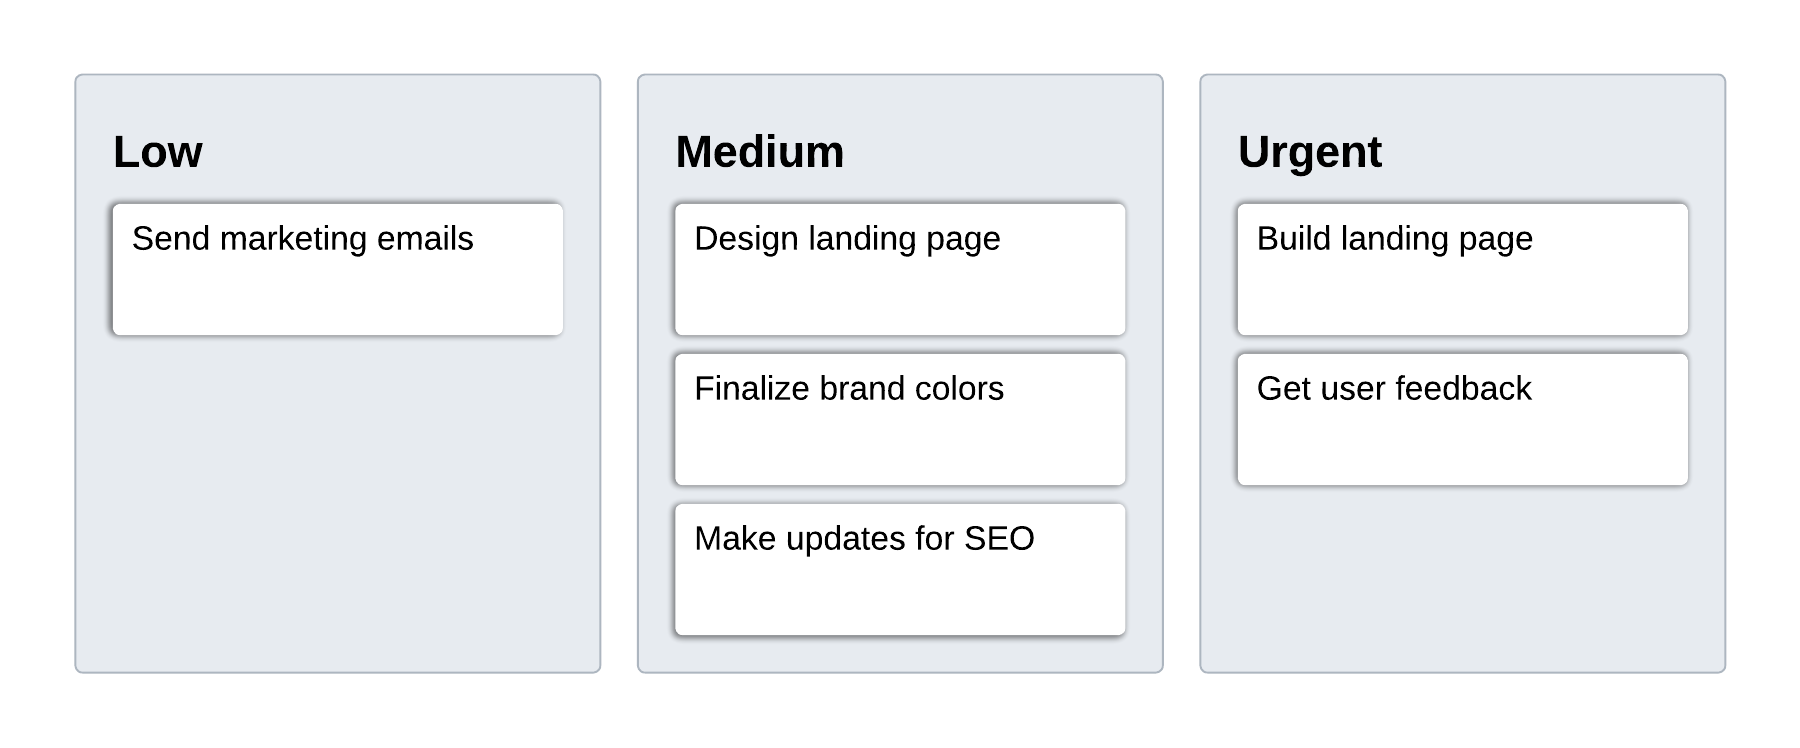
\includegraphics[width=0.8\textwidth]{diagrams/ebql-architecture.png}
    \caption{The eBQL system architecture. eBQL transforms an extended-SQL query into an abstract
    syntax tree, analyzes the query, then generating an eBPF program to execute the query. The
    program is then loaded into the kernel, and post-processed HFT data is streamed to the user.}
    \label{fig:ebql-architecture}
\end{figure}
eBQL transforms high-level extended-SQL queries through a series of steps before generating an eBPF
tracing program, loading it into the kernel, and streaming output results to the user (Figure
\ref{fig:ebql-architecture}). Crucially, the internals of eBPF is abstracted away from the user,
enabling HFT data collection in a declarative manner.

\subsection{eBQL API}
\label{ebql-api}

From a client perspective, eBQL exposes a simple query executor API with just two methods beyond a
default initialization: % (Figure \ref{code:ebql-api}).

% \begin{figure}[htpb]
\begin{lstlisting}
pub struct Executor {
    /// internal fields
}

impl Executor {
    /// Initializes an empty query executor.
    pub fn new() -> Executor;

    /// Executes an extended-SQL query.
    pub fn execute_query(
        &mut self,
        sql_query: String,
    ) -> Result<(Arc<Schema>, Receiver<RecordBatch>)>;

    /// Fetches the stats of a specific query.
    pub fn get_query_stats(&self, q: String) -> Option<QueryStats>;
}
\end{lstlisting}
% \caption{The eBQL API.}
% \label{code:ebql-api}
% \end{figure}

After initializing with \texttt{Executor::new()}, the executor takes in an extended-SQL query
(\S \ref{query-language}) and converts it into an eBPF instrumentation program executing in the
kernel. If successful, the executor returns the query's schema definition (\S 
\ref{data-rep-out}), and a receiver channel of streamed record batches (i.e., HFT data after being
processed by the query).


\subsection{Query Language}
\label{query-language}

To enable declarative querying, eBQL exposes a query language lightly extended from SQL.

At its core, eBQL supports the standard SQL functionality, using its relational operator set to
express typical data manipulation. However, eBQL extends standard SQL to support streaming semantics
using a \texttt{Window} operator, and adds additional support for time-series analysis via
histograms and quantiles (Table \ref{tab:ebql-ops} provides a complete operator list). In addition,
eBQL expands SQL’s syntax slightly to accommodate for the kernel event format.

\begin{table}[htpb]
    \centering
    \caption{Operators used in eBQL query plans.}
    \label{tab:ebql-ops}
    \begin{tabular}{|l|p{0.8\linewidth}|}
        \hline
        \multicolumn{1}{|c|}{\textit{\textbf{Operator}}} &
        \multicolumn{1}{c|}{\textit{\textbf{Description}}}
        \tabularnewline \hline
        Select & Selects a stream from a kernel tracing event, such as
        \texttt{tracepoint/filemap/mm\_filemap\_add\_to\_page\_cache}. \\
        \hline
        Window & Partitions unbounded streams into bounded relations, either by \texttt{time} or
        tuple \texttt{count}. Windows have a \texttt{step} value (either some time interval or
        tuple amount) $\le $ the window size.\\
        \hline
        Project & Selects specific attributes from a stream/relation. These attributes may be
        event-specific (e.g. \texttt{pfn} for page cache evictions), or generic system attributes
        (e.g. \texttt{pid/tgid}, \texttt{cgroup}, or CPU/SMP id).\\
        \hline
        Filter & Filters attributes based on some conditional statement, such as \texttt{pid ==
        12000}, or \texttt{count >= 4096}. \\
        \hline
        Map & Maps attributes from one value to another. Example maps use basic arithmetic (e.g.
        \texttt{count * 2}) or available BPF helper functions (e.g.
        \texttt{bpf\_get\_ns\_current\_pid\_tgid(dev, ino)}). \\
        \hline
        GroupBy & Groups events according to a set of grouping keys (e.g. \texttt{(fd, cpu)}).\\
        \hline
        Aggregate & Performs some aggregation over grouped elements. Supported aggregations are
        \texttt{max}, \texttt{min}, \texttt{sum}, \texttt{average}, \texttt{count},
        (linear/exponential) \texttt{histogram}s, and \texttt{quantile}s. \\
        \hline
        Distinct & Eliminates duplicates according to the group by key, preserving the most recent
        event. \\
        \hline
        Join & Joins two event streams by some specified condition (e.g. \texttt{A.pid == B.pid}).\\
        \hline
    \end{tabular}
\end{table}

The design of eBQL's query language is heavily inspired by the Continuous Query Language (CQL) from
Stanford's Data Stream Management System (ref: STREAM, CQL).

The kernel event is initially represented as a \textit{stream} ordered by some time domain (in this
context, the \texttt{ktime == clock\_gettime(CLOCK\_MONOTONIC)}). The \texttt{Window} operator can
then convert the kernel event stream into a bounded \textit{relation} by providing a sliding window
over the stream. eBQL's operators can operate on streams and/or relations, depending on their type:
\begin{itemize}
    \item Stateless operators like project, filter, and map can operate on either streams or
        relations, as each operates only on individual events and thus do not require some bounded
        amount of events to compute.
    \item Ungrouped stateful aggregations can operate on streams, accumulating values until the
        query is finished. This is permitted due to the minimal amount of state needed to store
        aggregation values: for instance, a \textit{count} aggregation without grouping requires
        only a constant amount of space---one \texttt{u64}---regardless of the amount of elements in
        the stream.
    \item Stateful (grouped) aggregations can also operate on bounded (i.e. windowed) relations.
        Data manipulation with these constructs perform the same functionality as their standard SQL
        equivalents: for instance, the \texttt{max} computed over a $1024$-count window is
        functionally equivalent to a \texttt{max} computed over a $1024$-row relation.
    \item Joins can only operate on relations: they must compute the result on the entire input
        before results are produced, so the input sources must be bounded relations, not unbounded
        streams.
\end{itemize}

From a user standpoint, besides from the additional \texttt{Window} operator to accommodate the
streaming nature of kernel events, eBQL's query language models the same semantics as standard SQL
with only slight syntactical differences.

As an example, Figure \ref{code:ebql-ex} shows a continuous aggregation query over \texttt{pread64}
syscall invocations.
\begin{figure}[htpb]
\begin{lstlisting}[language=SQL]
SELECT fd, cpu, COUNT(*), MAX(count), AVG(count)
    FROM tracepoint/syscalls/sys_enter_pread64
    GROUP BY fd, cpu
    WHERE pid == 1041370
    WINDOW(time, 1000, 1000);
\end{lstlisting}
\caption{A continuous eBQL aggregation query. The additional \texttt{Window} operator converts the
event stream into a relation: the first argument takes in the window type (\texttt{time} or
\texttt{count}), the second argument the interval, and the third argument the step size (for time,
in milliseconds).}
\label{code:ebql-ex}
\end{figure}

The query establishes a tumbling 1 second \texttt{time} window over the \texttt{sys\_enter\_pread64}
tracepoint, filters for syscalls from only the specified \texttt{pid} (here \texttt{1041370}), then
groups all invocations on the same \texttt{fd} and from the same \texttt{cpu}, and computes three
aggregations: the total number of elements, the maximum number of bytes read, and the average amount
of bytes read (for context, \texttt{count} in the \texttt{pread64} syscall represents the amount of
bytes to read).

The query then returns events every time the window steps forward (here, every second) as a
\texttt{RecordBatch} (Section \ref{data-rep-out}).

\subsection{Data Representation}
\label{data-rep}

\subsubsection{Relational Model}
Within eBQL, each kernel event is modeled as a \textit{streaming relation} with a fixed set of
attributes.

The existing kernel infrastructure inherently exposes a relational structure for its tracing events:
all (raw) tracepoints follow a fixed format (in Linux, defined at
\texttt{/sys/kernel/tracing /events/<category>/<name>/<format>}), while u[ret]probes and k[ret]probes
expose some probe-specific context with a general fixed structure. Thus, overlaying a relational
structure on top of kernel events provides almost a direct mapping from internal kernel
representations.

Selecting from a kernel event is then semantically equivalent to selecting from a data stream with a
fixed relational definition. For example, the \texttt{sys\_enter\_pread64} tracepoint (with
definition in Figure \ref{code:pread64-format}) is modeled as a relation with four fields,
\texttt{fd}, \texttt{buf}, \texttt{count}, and \texttt{pos} (which are also the arguments to
\texttt{pread64} (ref: pread64 manpage)). 

\begin{figure}[htpb]
\begin{lstlisting}[language=C]
name: sys_enter_pread64
ID: 697
format:
    // Four other fields, prefixed common_<field>, exist, but are not available to eBPF programs attached to tracepoints, and are thus omitted.
    field:int __syscall_nr; offset:8;   size:4; signed:1;
    field:unsigned int fd;  offset:16;  size:8; signed:0;
    field:char * buf;   offset:24;  size:8; signed:0;
    field:size_t count; offset:32;  size:8; signed:0;
    field:loff_t pos;   offset:40;  size:8; signed:0;
\end{lstlisting}
\caption{The \texttt{sys\_enter\_pread64} tracepoint definition, from
\texttt{/sys/kernel/tracing/events/syscalls/sys\_enter\_pread64/format}.}
\label{code:pread64-format}
\end{figure}

However, there are some important caveats to the relational model.

First, an event's context alone does not fully represent the context available. At each event, the
kernel exposes a generic set of system values (included, but not limited to, \texttt{ktime},
\texttt{pid/tgid}, \texttt{cgroup}, \texttt{cpu}, \texttt{comm}, and \texttt{task}).  Thus, in
addition to the event-specific context, each event's relational model additionally exposes a fixed
set of system attributes.

Second, many events contain complicated kernel structures. The system \texttt{task} struct is a
huge, deeply nested, struct; and in \texttt{block} IO tracepoints, the \texttt{request} struct
(Figure \ref{code:request-struct}) contains copious amounts of information, such as the
\texttt{gendisk}, \texttt{block\_device}, and more metadata.  To represent and access this data, the
relation contains a type resembling SQL's \texttt{STRUCT} complex type. 

\begin{figure}[htpb]
\begin{lstlisting}[language=C]
struct request {
    // ... additional fields ...  
    struct gendisk *rq_disk;
    struct block_device *part;
    u64 alloc_time_ns;
    u64 start_time_ns;
    u64 io_start_time_ns;
    short unsigned int wbt_flags;
    short unsigned int stats_sectors;
    // ... additional fields ...  
}
\end{lstlisting}
\caption{The \texttt{struct request} type at \texttt{block} IO tracepoints. Access would then
require nested de-references; for instance, accessing the first minor device number of a block IO
request would be \texttt{request.rq\_disk.first\_minor}.}
\label{code:request-struct}
\end{figure}

Because of these two cases, the event relational model is, in a sense, \textit{denormalized}. Each
relation contains attributes that are not specific to them, but rather available at many relations:
every relation contains generic system attributes, and for similar tracepoints (like the
\texttt{block} IO ones), each context contains ``duplicate'' attribute definitions for identical
structs.

However, this denormalization does not impose additional access or storage overhead. Each event
stream does not literally store all attributes in memory; rather, on every invocation, the BPF
program has \textit{read-only access} to contexts stored in \textit{existing} kernel memory,
requiring no additional storage. For instance, each process already has a \texttt{task} struct
associated with it in the kernel, and \texttt{block} IO requests already require a \texttt{request}
struct to be created somewhere in-kernel.

\subsubsection{Query Output}

Each query projects some subset of a kernel event and optionally performs some
aggregations/transformations on the data. To provide a structured representation, the query output
is represented as a \texttt{RecordBatch}:
\begin{lstlisting}
pub struct RecordBatch {
    pub schema: Arc<Schema>,
    pub records: Vec<Record>,
}
\end{lstlisting}

Each record batch contains the query's output \texttt{Schema} with a fixed set of
\texttt{DataType}s, with a collection of \texttt{Record}s representing the actual
\texttt{DataValue}s of each output record. \texttt{RecordBatch}es are streamed from queries whenever
the window steps forward.

The \texttt{RecordBatch} structure is intentionally modeled after existing database libraries'
representations, like \texttt{sqlx} (ref: sqlx) and Apache Arrow (ref: arrow).

\label{data-rep-out}

\subsection{Query Plans}

Given an extended-SQL query, eBQL then compiles it into a \textit{query plan} that represents the
query procedure. The conceptual query plan is again inspired heavily by CQL's design (ref: CQL).

Each query plan is composed of eBQL operators, similar to SQL query plans. For instance, the query
in Figure \ref{code:ebql-ex} has the following logical plan:

\begin{lstlisting}[language=C]
Select(tracepoint/syscalls/sys_enter_pread64)
    .Window(time, 1000ms, 1000ms)
    .Project(fd, cpu, count, pid, time)
    .Filter(pid == 1041370)
    .GroupBy(fd, cpu)
    .Aggregate(Count)
    .Aggregate(Max, count)
    .Aggregate(Average, count);
\end{lstlisting}

Conceptually, new events flow between operators via \textit{queues} that store intermediate results
between operators, and stateful operators store persistent values in \textit{synopses}. On window
steps, results stored in synopses are emitted, and expired events again flow through operators,
clearing themselves from any synopses that contain their state.

\subsubsection{Physical Plan and Query Optimization}

The physical implementation of a query plan is split into two components, the \textit{kernel-space}
and \textit{user-space} component. A key consideration is determining when to emit to user-space, as
communicating values from kernel-space to user-space incurs substantial overhead.

Specifically, eBPF programs emit values to user-space through a concurrent MPSC ring buffer
implemented as a BPF map (\texttt{BPF\_MAP\_TYPE\_RINGBUF}), which is consumed by a user-space
process. Much work has been done to optimize the data transmission, with memory-mapped pages
available to user-space applications to avoid kernel-to-user copying and support for \texttt{epoll}
or busy polling (ref: linux ringbuf docs). However, the context switching from user to kernel space,
synchronization and locking overhead of the ringbuf, and interrupt request work processing required
for polling, and more incur prohibitive overhead (we later evaluate these claims in
\S\ref{perf-drilldown}).

Thus, eBQL attempts to process records entirely in kernel space, emitting only the final results, as
this reduces the total number of events that must be emitted between kernel to user space. For now,
eBQL's query planning places any operator that can feasibly be implemented within eBPF's constraints
into kernel space, only deferring to user-space when an operator is not possible in kernel space.
Specifically, all operators except for general Joins and non-tumbling time windows are implemented
purely in kernel space (because eBPF does not have dynamic memory or non-constant-bounded loops,
Joins and non-tumbling time windows---which require unbounded loops---cannot currently be
implemented in eBPF).

Beyond the user-kernel space split, eBQL also performs standard logical query optimizations, such as
predicate pushdown, split conjunctive predicates, and projection pushdown (ref: pred pushdown).
Although BPF programs are not querying external storage---and thus materializing records/attributes
and its associated IO cost is not a factor---minimizing attribute materialization still provides
potentially significant performance benefits. This is because BPF programs do not have direct access
to all kernel memory; thus, system attributes require BPF helper functions to access such as
\texttt{bpf\_ktime\_get\_ns}---which can incur non-trivial overhead---and reading certain kernel
memory requires the \texttt{bpf\_probe\_read\_kernel} helper function, incurring significant
overhead due to memory copying and a dependency on variable arguments that requires runtime checks
for safety (ref: ebpf runtime policies, bpf probe read kernel source).

eBQL also takes advantage of the restriction to tumbling windows in eBPF to simplify windowing and
aggregation logic. In tumbling windows, every window step discards every element in the previous
window; thus, windowing needs only to record a constant amount of metadata to determine when to
tumble (e.g. items seen for count-based windows, or the start timestamp for time-based windows), and
every stateful operator simply clears its synopses, an almost-constant time operation (eBPF does not
support clearing maps in kernel-space, so it requires a map iteration to delete each element;
however, when values are grouped, the number of group-by keys is often significantly less than the
total amount of elements).

Currently, eBQL only employs rule-based optimization. However, recent work attempts to quantify the
cost of BPF operations (ref: ebpf runtime policies); thus, future work can explore estimates using
data characteristics to perform cost-based optimizations. For instance, if an eBPF operator requires
a high amount of costly function invocations or redundant memory allocation in BPF maps, it might be
more optimal to incur the kernel-user data transmission overhead and defer computation to user
space.

Operator implementations in user-space follow standard database operator implementations (for
instance, a Join could be implemented as a grace hash join or index nested loop join), and are thus
elided.

\subsection{Code Generation}

After processing the query plan, eBQL converts the kernel-space operators into BPF C code.

\texttt{bpftrace} implements a full fledged AST-LLVM IR-eBPF bytecode transformation pipeline;
however, \texttt{bpftrace} aims to support arbitrary procedural logic (an example is Figure
\ref{code:bpftrace-ex}). Due to the constrained set of operators available in eBQL, it opts for a
simpler approach of composing together multiple operator representations and generating a collection
of output header files, with struct, map, and operator definitions in C, included into one source
file (details can be found in \S\ref{impl-codegen}).

The generated C code is then dispatched to \texttt{clang}, which compiles it down into eBPF
bytecode.

\subsection{Query Execution and Post-Processing}

eBQL then loads the generated eBPF bytecode into the kernel, where the eBPF verifier checks the
query for validity (because eBQL's internal catalog should handle logical bindings, and the codegen
step should properly adhere to eBPF requirements, users are abstracted away from verifier
peculiarities; failure at the verifier indicates a bug in eBQL itself, not in the user query).

eBQL then processes the loaded BPF objects, setting global flags and optionally pinning maps (a
feature useful for synopsis sharing, but not currently implemented by eBQL) before attaching the
program to the kernel event. At this point, the generated BPF program is now running in the kernel,
and query output is streamed to the user.

% \subsection{References}
% \begin{itemize}
    % \item STREAM: data stream management book
    % \item CQL
    % \item sqlx: https://docs.rs/sqlx/0.7.4/sqlx/trait.Database.html\#associatedtype.QueryResult
    % \item apache arrow: https://arrow.apache.org/rust/arrow/record\_batch/struct.RecordBatch.html
    % \item linux ringbuf docs: https://docs.kernel.org/bpf/ringbuf.html
    % \item pred pushdown: https://www.vldb.org/conf/1994/P096.PDF
    % \item bpf runtime policies: https://people.cs.vt.edu/djwillia/papers/ebpf23-runtime.pdf
    % \item bpf probe read kernel source:
        % https://elixir.bootlin.com/linux/v6.7/source/include/linux/bpf.h\#L2742
% \end{itemize}
